\vspace{-0.1cm}
\begin{figure*}[tb]
    \centering
    \setlength{\belowcaptionskip}{-5pt}
    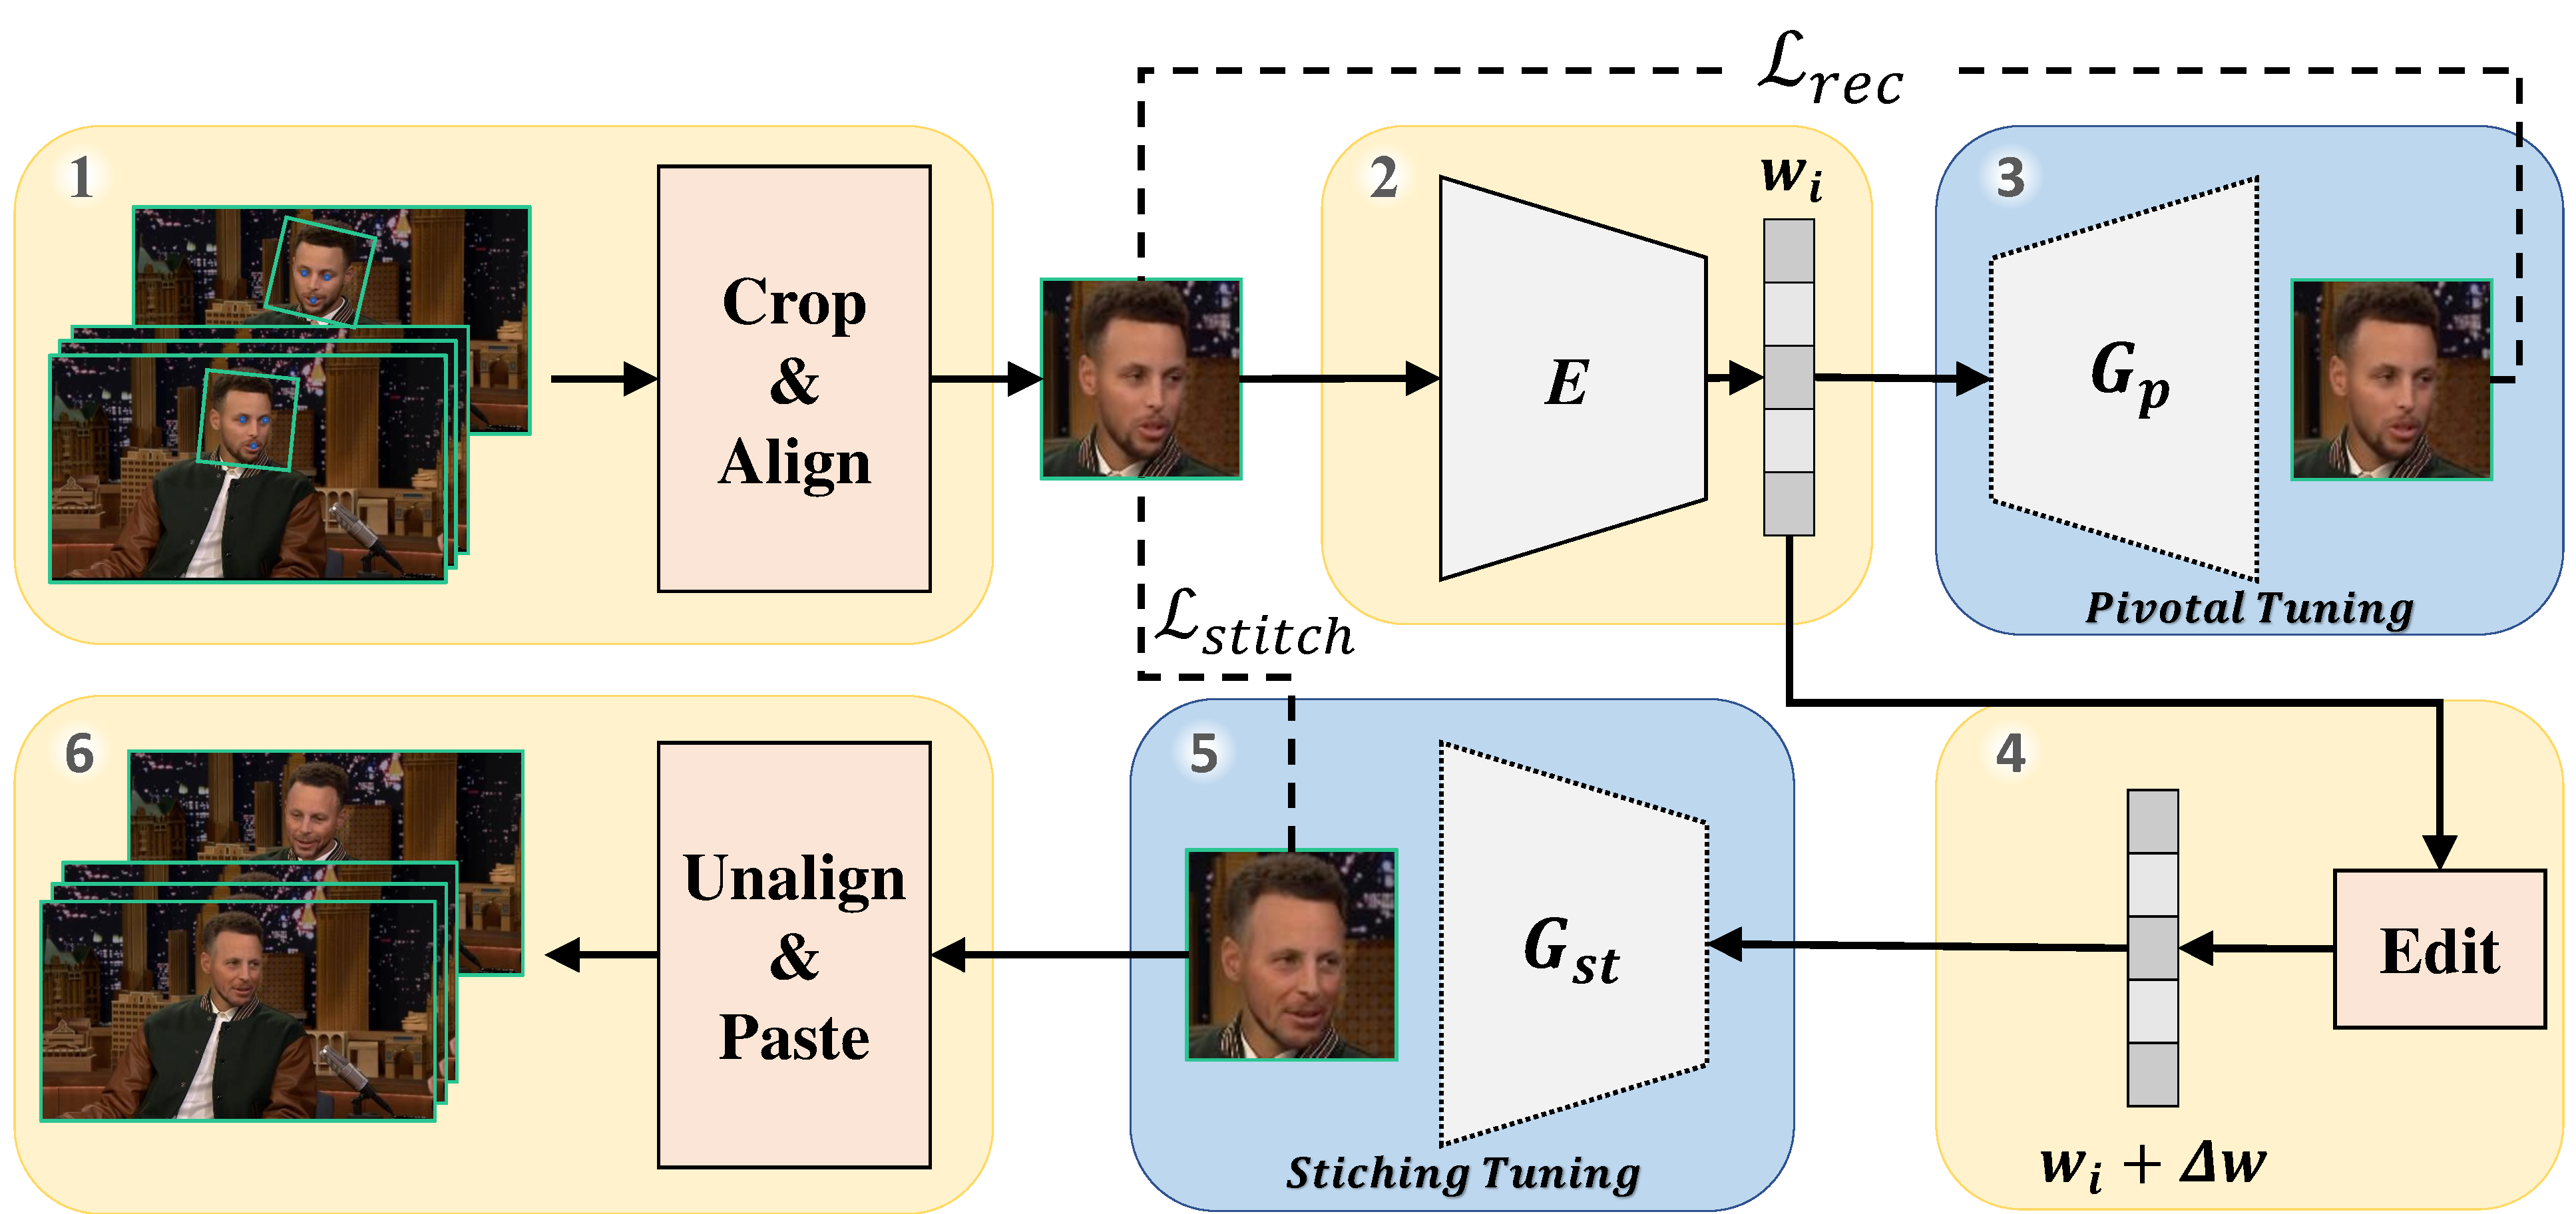
\includegraphics[width=0.97\linewidth]{resources/images/pipeline.pdf}
    % \vspace{-0.25cm}
    \caption{
    Our full video editing pipeline contains $6$ steps. $(1)$ Videos are split into individual frames. The face in each frame is cropped and aligned. $(2)$ Each cropped face is inverted into the latent space of a pre-trained StyleGAN2 model, using a pre-trained e4e encoder. $(3)$ The generator is fine-tuned using PTI across all video frames in parallel, correcting for inaccuracies in the initial inversion and restoring global coherence. $(4)$ All frames are edited by manipulating their pivot latent codes linearly, using a fixed direction and step-size. $(5)$ We fine-tune the generator a second time, stitching the backgrounds and the edited faces together in a spatially-smooth manner. $(6)$ We reverse the alignment step and paste the modified face into the video.
    }
    % \vspace{-0.1cm}
    \label{fig:pipeline}
\end{figure*}